%%%
% Plantilla de Memoria
% Modificación de una plantilla de Latex de Nicolas Diaz para adaptarla 
% al castellano y a las necesidades de escribir informática y matemática%
% Editada por: Mario Román
%
% License:
% CC BY-NC-SA 3.0 (http://creativecommons.org/licenses/by-nc-sa/3.0/)
%%%

%%%%%%%%%%%%%%%%%%%%%%%%%%%%%%%%%%%%%%%%%
% Thin Sectioned Essay
% LaTeX Template
% Version 1.0 (3/8/13)
%
% This template has been downloaded from:
% http://www.LaTeXTemplates.com
%
% Original Author:
% Nicolas Diaz (nsdiaz@uc.cl) with extensive modifications by:
% Vel (vel@latextemplates.com)
%
% License:
% CC BY-NC-SA 3.0 (http://creativecommons.org/licenses/by-nc-sa/3.0/)
%
%%%%%%%%%%%%%%%%%%%%%%%%%%%%%%%%%%%%%%%%%

%----------------------------------------------------------------------------------------
%	PAQUETES Y CONFIGURACIÓN DEL DOCUMENTO
%----------------------------------------------------------------------------------------

%%% Configuración del papel.
% microtype: Tipografía.
% mathpazo: Usa la fuente Palatino.
\documentclass[a4paper, 20pt]{article}
\usepackage[a4paper,margin=1in]{geometry}
\usepackage[protrusion=true,expansion=true]{microtype}
\usepackage{mathpazo}

% Indentación de párrafos para Palatino
\setlength{\parindent}{0pt}
  \parskip=8pt
\linespread{1.05} % Change line spacing here, Palatino benefits from a slight increase by default


%%% Castellano.
% noquoting: Permite uso de comillas no españolas.
% lcroman: Permite la enumeración con numerales romanos en minúscula.
% fontenc: Usa la fuente completa para que pueda copiarse correctamente del pdf.
\usepackage[spanish,es-noquoting,es-lcroman,es-tabla,,es-nodecimaldot]{babel}
\usepackage[utf8]{inputenc}
\usepackage{fontenc}
\selectlanguage{spanish}


%%% Gráficos
\usepackage{graphicx} % Required for including pictures
\usepackage{wrapfig} % Allows in-line images
\usepackage[usenames,dvipsnames]{color} % Coloring code
%\usepackage{subcaption}
\usepackage{subfig}
\graphicspath{{media/}}


%%% Matemáticas
\usepackage{amsmath}
\usepackage{physics} % para las derivadas parciales
\usepackage[Symbol]{upgreek} %pi

%%% Pseudocódigo

\usepackage[htt]{hyphenat}
\usepackage{algorithmicx}
\usepackage[ruled]{algorithm}
\usepackage{algpseudocode}

\newcommand{\alg}{\texttt{algorithmicx}}
\newcommand{\old}{\texttt{algorithmic}}
\newcommand{\euk}{Euclid}
\newcommand\ASTART{\bigskip\noindent\begin{minipage}[b]{0.5\linewidth}}
\newcommand\ACONTINUE{\end{minipage}\begin{minipage}[b]{0.5\linewidth}}
\newcommand\AENDSKIP{\end{minipage}\bigskip}
\newcommand\AEND{\end{minipage}}

%%% Código
\usepackage{listings}
\lstset{
  basicstyle=\ttfamily,
  columns=fullflexible,
  %frame=single,
  breaklines=true
}

%%% Tablas
\usepackage{tabularx}
\usepackage{float}
\usepackage{adjustbox}
\usepackage{booktabs}

% Enlaces y colores
\usepackage{hyperref}
\usepackage[dvipsnames]{xcolor}
\definecolor{webgreen}{rgb}{0,0.5,0}
\hypersetup{
  colorlinks=true,
  citecolor=RoyalBlue,
  urlcolor=RoyalBlue,
  linkcolor=RoyalBlue
}

%%% Bibliografía
\usepackage[backend=biber]{biblatex}
\addbibresource{citations.bib}


\newcommand{\training}{\textit{training }}
\newcommand{\test}{\textit{test }}
\newcommand{\R}{\mathbb R}

%%% Subsubsection con letras
\renewcommand{\thesubsubsection}{\thesubsection.\alph{subsubsection}}

%%% Itemize, enumitem
\usepackage{paralist}
\usepackage{enumitem}
%----------------------------------------------------------------------------------------
%	TÍTULO
%----------------------------------------------------------------------------------------
% Configuraciones para el título.
% El título no debe editarse aquí.
\renewcommand{\maketitle}{
  \begin{flushright} % Right align
  
  {\LARGE\@title} % Increase the font size of the title
  
  \vspace{50pt} % Some vertical space between the title and author name
  
  {\large\@author} % Author name
  \\\@date % Date
  \vspace{40pt} % Some vertical space between the author block and abstract
  \end{flushright}
}

%% Título
\title{\textbf{Título}\\ % Title
Subtítulo} % Subtitle

\author{\textsc{Autor1,\\Autor2} % Author
\\{\textit{Universidad de Granada}}} % Institution

\date{\today} % Date

%-----------------------------------------------------------------------------------------
%	DOCUMENTO
%-----------------------------------------------------------------------------------------

\begin{document}

%-----------------------------------------------------------------------------------------
%	TITLE PAGE
%-----------------------------------------------------------------------------------------

\begin{titlepage} % Suppresses displaying the page number on the title page and the subsequent page counts as page 1
	
	\raggedleft % Right align the title page
	
	\rule{1pt}{\textheight} % Vertical line
	\hspace{0.05\textwidth} % Whitespace between the vertical line and title page text
	\parbox[b]{0.8\textwidth}{ % Paragraph box for holding the title page text, adjust the width to move the title page left or right on the page
		
		{\Huge\bfseries Práctica 3\\[0.5\baselineskip]\large Ajuste de datos usando modelos lineales\\[2\baselineskip]} % Title
		{\large\textit{\today}\\[0.5\baselineskip]Aprendizaje Automático\\[1.5\baselineskip] }% Subtitle or further description
		{\Large\textsc{Francisco Javier Sáez Maldonado}\\[0.5\baselineskip]fjaviersaezm@correo.ugr.es} % Author name, lower case for consistent small caps
		
		\vspace{0.4\textheight} % Whitespace between the title block and the publisher
		
		{\noindent \\[0.5\baselineskip] }\\[\baselineskip] % Publisher and logo
	}

\end{titlepage}

%% Resumen (Descomentar para usarlo)
%\renewcommand{\abstractname}{Resumen} % Uncomment to change the name of the abstract to something else
%\begin{abstract}
% Resumen aquí
%\end{abstract}

%% Palabras clave
%\hspace*{3,6mm}\textit{Keywords:} lorem , ipsum , dolor , sit amet , lectus % Keywords
%\vspace{30pt} % Some vertical space between the abstract and first section


%% Índice
{\parskip=2pt
  \tableofcontents
}
\pagebreak

\section*{Introducción}

En esta práctica, trataremos de realizar un estudio completo de un problema en el que se nos
presenta un conjunto de datos y nuestro objetivo es seleccionar el mejor predictor lineal para
este conjunto de datos dado. Concretamente, estudiaremos dos conjuntos de datos extraidos
de la web \href{https://archive.ics.uci.edu/ml/index.php}{UCI-Machine Learning Repository}.

Utilizaremos uno de ellos para tratar de ajustar un modelo lineal a un problema de regresión, y otro conjunto diferente de datos para ajustar otro modelo lineal a un problema de clasificación multiclase. El objetivo será realizar un estudio de los datos, evitando en todo momento el \emph{data snooping}, y argumentar si se utilizan ciertas técnicas de preprocesado de datos antes de escoger el modelo final.

Trataremos primero el problema de regresión y posteriormente el de clasificación.

\section{Regresión}

\subsection{Estudio del conjunto de datos. Identificación de $\mathcal X,\mathcal Y,f$.}

Lo primero que debemos hacer es realizar una buena comprensión de la información que tenemos sobre los datos para comprender un poco más nuestro problema.

Nuestro primer conjunto de datos, \cite{superdata}, contiene características de ciertos elementos superconductores. Junto con estas características, se nos presenta una \emph{temperatura crítica}, que en el artículo en el que se estudia el conjunto de datos de manera más profunda \cite{hamidieh} lo denominan $T_c$, obtenida para un superconductor que posea estas características. También se nos presenta un archivo en el que se nos dan las fórmulas químicas de los superconductores, pero este archivo no será relevante para nosotros.

Lo primero que nos encontramos acerca de nuestros datos es la siguiente tabla:
\begin{table}[h]
  \centering
  \begin{tabular}{|l|l|l|l|}
    \hline
    Características         & Multivariable & Número de instancias & $21263$ \\ \hline
    Tipo de características & Reales        & Número de atributos  & $81$    \\ \hline
    Tareas asociadas        & Regresión     & Valores perdidos     & $N\backslash A$   \\ \hline
  \end{tabular}
  \caption{Datos contenidos en el conjunto de datos Superconductivity.}
\end{table}


Esta información nos resulta muy útil, pues obtenemos podemos observar que tenemos $81$ atributos para cada una de las $21263$ instancias. De aquí podemos obtener que el tamaño del conjunto de datos es bastante amplio, por lo que tendremos un buen conjunto de entrenamiento. Las características que obtenemos son reales, es decir, $x_i \in \mathbb R^{81}$. Para completar, vemos que no tenemos valores perdidos, por lo que nos ahorraremos en este caso tener que establecer una técnica para reconstruir estos valores.

Con la información proporcionada podemos decir que:

\begin{enumerate}
\item Nuestro conjunto de datos de entrenamiento será
  $$\mathcal X = \{ X_i \in \R^{81}, \text{ con } i = 1, \dots , 21263 \}.$$

\item Nuestro conjunto de etiquetas, puesto que no se nos indica ninguna restricción sobre las temperaturas, podemos asumir que es:
  $$
  \mathcal Y = \{ y_i \in \R, \text { con } i = 1,\dots,21263\}.
  $$

\item Por último, nuestra función $f : \mathcal X \to \mathcal Y$ que asigne a cada vector de características una temperatura crítica.
  
\end{enumerate}

Hay que anunciar que los siguientes gráficos de visualizado de datos se han realizado posteriormente a realizar la separación en conjuntos de \emph{train} y \emph{test} de nuestro conjunto de datos, para evitar en todo momento el \emph{data snooping}.\\

Dibujamos ahora un gráfico en el que mostramos el diagrama de caja de los posibles valores que toma la temperatura $T_c$:

\begin{figure}[H]
  \centering
  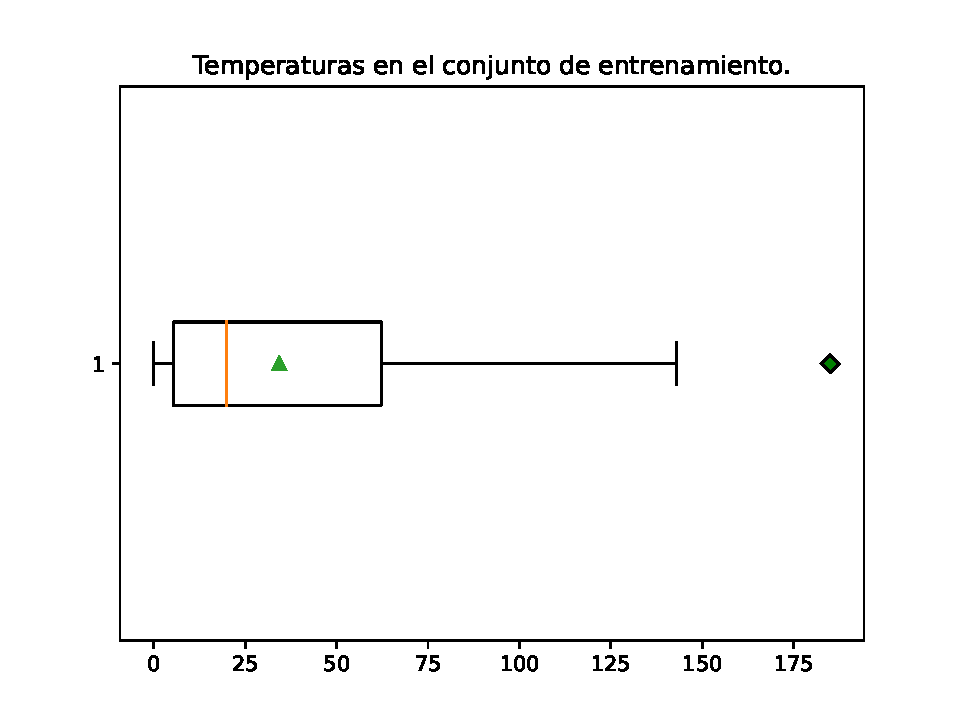
\includegraphics[scale = 0.4]{boxplot_y.pdf}
  \caption{Diagrama de caja de las temperaturas $T_c$ en el conjunto de entrenamiento.}
\end{figure}

Como podemos ver, aunque tenemos variabilidad en los valores de $f$, tenemos la mayoría de estos concentrados en el intervalo $[0,50]$, lo cual nos indica que hay probabilidad de que los datos no sean separables o tengamos ruido en nuestra muestra. Como podemos ver, tenemos un dato que se aleja mucho de $1.5$ por el rango intercuartílico, que es lo que representan los \emph{bigotes} del diagrama de caja. Es por ello que podemos decir que este punto es posiblemente un \emph{outlier}.

En cuanto a los valores de nuestros datos, si tomamos el primer elemento y calculamos la desviación típica $\sigma$ y el resultado que obtenemos es:
\begin{lstlisting}[lang = Python]
  Standard deviation of the first element of the dataset 2747.992
\end{lstlisting}
Por lo que obtenemos que claramente los valores de los diferentes atributos no están en el mismo rango de escala. Es por ello que previamente al entrenamiento realizaremos una estandarización por atributos de nuestro conjunto de datos.

\newpage
\printbibliography

\end{document}
